% !TeX program = xelatex
\documentclass[10pt, a4paper]{article}
\usepackage[titles]{tocloft}

% Document information
\newcommand{\thetitle}{Thesis}
\title{\thetitle}
\author{Chair for Information Systems and AI in Marketing}
\date{\today}


% Font (Verdana only usable with XeLaTeX Compiler instead of pdfLaTeX)
\usepackage{fontspec}
\setmainfont{Verdana}


\usepackage[american]{babel}
\addto\captionsamerican{% Replace "english" with the language you use
  \renewcommand{\contentsname}%
    {Table of Contents}%
}



\usepackage{csquotes}
\usepackage{array}
\usepackage{parskip}



%\newfontfamily\Verdana{Verdana}[Scale=MatchLowercase, Ligatures=TeX]
\newfontfamily\Verdana{Verdana}[Ligatures=TeX]
%\newfontfamily\Arial{Arial}[Ligatures=TeX]


% Headers
\usepackage{titlesec}

%\titlespacing{\section}{0pt}{2pt}{6pt}{0pt}

\titleformat{\section}
{\bfseries\fontsize{16pt}{18pt}\selectfont}
{\thesection}{1em}{}

\titleformat{\subsection}
{\bfseries\fontsize{14pt}{16pt}\selectfont}
{\thesubsection}{1em}{}

\titleformat{\subsubsection}
{\bfseries\fontsize{12pt}{14pt}\selectfont}
{\thesubsubsection}{1em}{}

% Read in template when to use subheadings 
\newcommand{\subheading}[1]{
  \par\noindent
  {\bfseries\fontsize{12pt}{14pt}\selectfont #1\par}
  \vspace{0.75em}
}

% References 
\usepackage[style=apa,backend=biber]{biblatex}
\addbibresource{references.bib}
% Distance between sources in references section
\usepackage{etoolbox}
\setlength\bibitemsep{1em}
\apptocmd{\bibsetup}{\setlength{\itemsep}{\bibitemsep}}{}{}

% For specifying the format of table of contents, list of figures and list of tables
% Without [titles here, the Table of Contents does not have a header]
\renewcommand{\cftdotsep}{0.5}
\renewcommand{\cftsecleader}{\cftdotfill{\cftdotsep}}
\renewcommand{\cftfigpresnum}{Figure~}
\renewcommand{\cftfigaftersnum}{: }


\settowidth{\cftfignumwidth}{Figure 99: }
\renewcommand{\cfttabpresnum}{Table~}
\renewcommand{\cfttabaftersnum}{: }
\settowidth{\cfttabnumwidth}{Table 99: }
\setlength{\cftsecindent}{0pt}% Remove indent for \section
\setlength{\cftsubsecindent}{0pt}
\setlength{\cftsubsubsecindent}{14pt}
\renewcommand{\tocloftpagestyle}{fancy}
\setlength{\cftfigindent}{0pt}  % remove indentation from figures in lof
\setlength{\cftafterloftitleskip}{400pt}
\setlength{\cfttabindent}{0pt}  % remove indentation from tables in lot
%\renewcommand{\tocloftpagestyle}{empty}




% To include graphics, specify the path to the images
\usepackage{graphicx}
\graphicspath{ {images/} }

% Package for better symbols 
\usepackage{pifont}

% Standardization of enumeration levels
\usepackage{enumitem}
\setlist[itemize,2]{label=\raisebox{-0.2ex}{\scalebox{1.5}{\textopenbullet}}}
\setlist[itemize,3]{label=\raisebox{0.3ex}{\scalebox{0.4}{\ding{110}}}}

% For tables
\usepackage{tabularx}
\usepackage{colortbl}
\usepackage[table]{xcolor}
\usepackage{longtable}
\usepackage{ltablex}
\keepXColumns
\usepackage{float}
\makeatletter
\@ifpackagelater{longtable}{2026/01/01}{}{
  \patchcmd{\LT@output}{\copy\LT@foot\vss}{\copy\LT@foot\vskip 0pt plus 1fil minus \normalbaselineskip}{}{}
  \patchcmd{\LT@output}{\copy\LT@foot\vss}{\copy\LT@foot\vskip 0pt plus 1fil minus \normalbaselineskip}{}{}
}
\makeatother

% For captions of figures and tables 
\usepackage{caption}
\captionsetup{
  font={bf,footnotesize},
  labelfont=bf,
  labelsep=colon,        
  textformat=simple      
}

% For correct placement of images on the title page
\usepackage{chngpage}
\usepackage{calc}
\usepackage{pgfgantt}
\usetikzlibrary{arrows.meta,positioning}

% Spacing
\usepackage{geometry}
\geometry{left=3cm, right=2cm, top=2.5cm, bottom=3cm, papersize={210mm, 297mm}}
%\geometry{papersize={210mm, 297mm}}
\usepackage{setspace}
%\onehalfspacing
%\setstretch{1.6}

% Header 
\usepackage{fancyhdr}
\usepackage{color}
% Page numbering and title 
\pagestyle{fancy}
\fancyhf{} 
\fancyhead[L]{[Titel]}
\fancyhead[R]{\thepage}
% Line in the header 
\renewcommand{\headrulewidth}{0.15pt}
\makeatletter
\renewcommand{\headrule}{%
  {\color{black}\hrule width\headwidth height\headrulewidth \vskip-\headrulewidth}
}
\makeatother
\setlength{\headwidth}{\textwidth}

% Automatic generation of hyperlinks for references (ref / cite)
\usepackage{hyperref}
\hypersetup{
  hypertexnames = false,
  colorlinks   = true,    % Colours links instead of ugly boxes
  urlcolor     = black,    % Colour for external hyperlinks
  linkcolor    =  black,    % Colour of internal links
  citecolor    = black      % Colour of citations
}

%\onehalfspacing
%\linespread{1.25}
%\linespread{1.028}
\setstretch{1.5}
%\usepackage[fontsize=10bp]{scrextend}
\usepackage{color, soul}

%\usepackage[english]{babel}

\newcolumntype{L}{>{\raggedright\arraybackslash}X}

\begin{document}
    \addtocontents{lof}{\vskip 14pt}
    \addtocontents{lot}{\vskip 14pt}
    %\addtocontents{lof}{\vskip 1.2cm}

    %\onehalfspacing
    \titlespacing{\section}{0pt}{2pt}{6pt}
    \titlespacing{\subsection}{0pt}{6pt}{6pt}
    \titlespacing{\subsubsection}{0pt}{6pt}{6pt}
    
    % Title in header (again for safety)
    \fancyhead[L]{[A Physio-Adaptive System for Real-Time Flow Detection in Competitive Esports]}
    
    % Title page
    

\begin{titlepage}
    \newgeometry{bottom=1cm}

    \thispagestyle{empty}

    % Banner oben
    \begin{picture}(0,0)(77,-10)
        
\includegraphics{images/UDE_header.png}
    \end{picture}
    \vspace{1.5cm}

    % Titel und Untertitel
    \begin{center}
        {\large \bfseries A Physio-Adaptive System for Real-Time Flow Detection in Competitive Esports}
        % Use this when your title requires 2 lines 
        % {\Huge \bfseries Fist line\\[0.3em] Second line}
        \\ %[1.2em]
        {\large Master thesis}
    \end{center}
    \vspace{2cm}
    
    % Linksbündige Infos
    \begin{center}
    \begin{flushleft}
    \begin{tabular}{p{0.4cm}p{6cm}p{9cm}}
        & Submitted by:      & Ahmed Mousa \\
        \rule{0pt}{18pt} & Address:  &   Hamborner Altmarkt 28 47166, Duisburg \\
        \rule{0pt}{18pt} & Study program:     & Master Computer Engineering  \\
        \rule{0pt}{18pt} & Matriculation number: & 3101343 \\
        \rule{0pt}{18pt} & First reviewer:   & Prof. Dr. Mario Nadj \\
        \rule{0pt}{18pt} & Second reviewer:   & Prof. Rothe  \\
        \rule{0pt}{18pt} & Delivery date   & 02.02.2027 \\
        \rule{0pt}{18pt} &  Semester of study  & Winter semester 2027, 9th Semester \\
    \end{tabular}
    \end{flushleft}
    \end{center}
    %\vfill
    \vspace{1cm}

    % Universität und Lehrstuhl unten
    \begin{center}
        University of Duisburg-Essen\\
        \vspace{0.4cm}
        Chair of Information Systems and Artificial Intelligence in Marketing\\
        \vspace{0.4cm}
        Faculty of Computer Science
    \end{center}

    % Banner unten
    \vspace{6.8cm}
    \begin{picture}(0,0)(77,0)
        
\includegraphics[width=1.362\textwidth]{images/Footer Thesis Template.png}
    \end{picture}

    \restoregeometry
\end{titlepage}
    \newpage

    \pagenumbering{roman}

    % Abstract
    \section*{Abstract (only for Bachelor/Master thesis)}
    \addcontentsline{toc}{section}{Abstract (only for Bachelor/Master thesis)}
        The abstract serves to give the reader a rough overview of the content (brief problem definition, solution approaches and possibly the key findings). 
\begin{itemize}[topsep=0pt,itemsep=-1ex,partopsep=0ex,parsep=1ex]
    \item The abstract should be a \textbf{maximum of half a page} in length. 
    \item The abstract should always be written in English. 
    \item This section must be deleted for seminar papers.
\end{itemize}


    \newpage
    
    % Table of Contents
    \setstretch{1.75}
    \thispagestyle{fancy}
    \fontsize{10pt}{10pt}\selectfont
    \tableofcontents
    \newpage
    \fontsize{10pt}{10pt}\selectfont
    \setstretch{1.5}
    

    % List of Abbreviations 
    \section*{List of Abbreviations\\(only for Bachelor/Master thesis)}
    \addcontentsline{toc}{section}{List of Abbreviations (only for Bachelor/Master thesis)}
        % List of Abbreviations placeholder\n\n

    \newpage    

    % Chapters
    \pagenumbering{arabic}   
    
    \section{Introduction}
        Electronic sports (e-sports) have grown into a major global domain, with industry reports describing a worldwide audience in the hundreds of millions and a market value above USD 2 billion \autocite{newzoo2024}. In this highly competitive context, the psychological state of \textit{flow} is considered a key performance factor. Within flow theory, flow emerges when perceived player skill and task challenge are well balanced \autocite{inbook,Moneta2012}. This thesis focuses on \textit{League of Legends} (LoL) as its specific e-sports context because LoL combines a large competitive ecosystem with clearly structured ranked tiers, team-based coordination, rapid decision-making, and frequent high-pressure events such as fights and objective contests \autocite{riotgames_lol,gong2020league,10.1145/3549506}. These characteristics make LoL a suitable case for examining how flow can be detected and protected in a demanding real-time game environment.

From a sensing perspective, the thesis places particular emphasis on electrocardiography (ECG). ECG-derived heart rate and heart rate variability (HRV) features provide a comparatively unobtrusive way to capture autonomic arousal and cognitive load during gameplay, and prior work has demonstrated that flow-related states can be classified from HRV-based physiological signals \autocite{9296229}. Because ECG can be recorded with a chest belt without requiring players to interrupt play or wear highly intrusive equipment, it is especially relevant for e-sports settings in which comfort, movement freedom, and competitive integrity are important. In addition to ECG, webcam-based facial recordings provide non-invasive affect-related cues that can be synchronized with gameplay and physiological data in gaming contexts \autocite{kutt2022biraffe2}. This combination motivates a practical sensing setup that links ECG-derived HRV features with webcam-based affect features for later live evaluation. This technical foundation supports the development of \textit{physio-adaptive systems} that use real-time physiological and affect-related data to infer user states and trigger digital environmental adaptations \autocite{irshad2023wearable,ubt_eref88160}.

Despite the demonstrated feasibility of physiological state detection, research regarding specialized interventions in the e-sports domain remains remarkably scarce. As shown by \cite{ubt_eref88160}, prior work has explored flow support through live biofeedback to enhance user awareness and emotion regulation during task execution. Likewise, \cite{9296229} demonstrated that binary flow states (high vs. low) can be classified from HRV using machine learning models. However, the unique demands of competitive LoL gameplay---characterized by extreme physiological arousal, rapid-fire decision-making, team communication, and specialized motor patterns---are not yet sufficiently addressed in these enterprise-focused approaches \autocite{banyai2019psychology,poulus2021determinants,10.1145/3549506}.


To address this gap, this thesis investigates the design requirements and technical implementation of a physio-adaptive system specifically tailored to protect and sustain flow in e-sports. By moving beyond general classification models, this study seeks to identify specialized, context-aware mechanisms that effectively assist e-sports athletes in maintaining peak performance. Accordingly, the study addresses the following research questions:

\begin{itemize}
    \item \textbf{RQ1:} How can ECG and webcam-based data be utilized to accurately distinguish between high and low flow states in a competitive LoL environment? \label{rq:classification}
    \item \textbf{RQ2:} What are the specific design requirements and intervention mechanisms for a physio-adaptive system that effectively assists LoL players in maintaining their flow state? \label{rq:adaptation}
\end{itemize}   

To answer these questions, the thesis follows a multi-phase mixed-methods design. First, a comprehensive baseline of system requirements is derived from the literature and a series of semi-structured interviews triangulated across three distinct cohorts: active competitive League of Legends (LoL) players, game design experts, and physiological computing specialists. These diverse empirical perspectives serve to identify context-aware adaptive measures for the e-sports environment, directly informing the development of a functional working prototype. During model development, the classification pipeline draws on multimodal training data and established physiological flow-classification frameworks \autocite{9296229,irshad2023wearable}. In the final live evaluation, however, the prototype is restricted to the signals available from the deployed setup---namely ECG-derived features and webcam-based features only. Finally, the prototype’s practical utility and the effectiveness of its adaptive interventions are evaluated through follow-up qualitative interviews and functional testing. Throughout the study, qualitative data are analyzed using Grounded Theory Methodology (GTM) \autocite{recker2021researchmethods} to anchor technical design decisions in the lived experiences and competitive requirements of the athletes \autocite{delveholempaecher2024openaxialselective}.

    \clearpage    
    \section{Foundation} 
        This chapter establishes the theoretical foundation of the thesis. It first introduces flow as a psychological state and explains it through the challenge-skill model. It then summarizes physiological and behavioral correlates of flow and motivates the biometric and webcam-based signals used in this work. Building on that basis, the chapter discusses physio-adaptive systems and their practical limitations. Finally, it presents the biocybernetic control loop as the guiding architecture for closed-loop human-computer interaction.

\subsection{The Phenomenon of Flow}

The concept of \enquote{flow}, first formalized by \textcite{inbook}, describes a state of \enquote{optimal experience} in which individuals are fully absorbed in an activity. In this state, action and awareness converge, self-referential thought recedes, and the subjective perception of time is altered \autocite{nah2014flow}. According to \textcite{inbook}, this state is defined by nine distinct dimensions that characterize the depth of the experience:

\begin{enumerate}
    \item \textbf{Challenge-Skill Balance:} The task's difficulty matches the individual's high level of skill.
    \item \textbf{Action-Awareness Merging:} The individual and the activity become one; movements feel automatic.
    \item \textbf{Clear Goals:} The user understands exactly what needs to be achieved at every step.
    \item \textbf{Unambiguous Feedback:} Performance success or failure is immediately apparent, allowing for real-time adjustment.
    \item \textbf{Concentration on the Task at Hand:} A high degree of focus that excludes all irrelevant thoughts or distractions.
    \item \textbf{Sense of Control:} The user feels a sense of agency and mastery over their actions and the environment.
    \item \textbf{Loss of Self-Consciousness:} The ego recedes, and the individual stops worrying about social evaluation.
    \item \textbf{Transformation of Time:} Time is perceived differently, either appearing to speed up or slow down significantly.
    \item \textbf{Autotelic Experience:} The activity is intrinsically rewarding, meaning it is performed for its own sake rather than for an external reward.
\end{enumerate}

A central explanatory framework for achieving these dimensions is the \textbf{challenge-skill model}. The model assumes that flow emerges in a \enquote{channel} where perceived task demands are well matched to an individual's capabilities. 



While the literature describes several alternative conceptualizations—including the eight-channel model, which segments the experience into states such as arousal and apathy, and the dynamic process approach, which views flow as a longitudinal path \autocite{Moneta2012}—this thesis specifically utilizes the challenge-skill model. This selection is grounded in the model's high degree of operational utility for physio-adaptive system design. Unlike more descriptive or longitudinal models, the challenge-skill framework can be operationalized either as a tertiary structure (Boredom vs. Flow vs. Anxiety) or as a binary classification problem. In the binary case, \textit{Flow} represents the positive class, while \textit{Boredom} and \textit{Anxiety} are grouped as \textit{non-flow} states. This makes the model well suited for real-time machine learning classification. Furthermore, it aligns with the principles of Dynamic Difficulty Adjustment (DDA) in e-sports, where the primary objective is to maintain the "Flow Channel" by balancing system demands against the player's physiological responses \autocite{Moneta2012, cowley2008understanding}.


As shown in Figure~\ref{fig:challengeSkillDiagram}, an imbalance in either direction tends to move users away from flow: excessive challenge relative to skill is associated with \textbf{anxiety}, while insufficient challenge is associated with \textbf{boredom}. In e-sports contexts, this relation is often interpreted as an information-processing fit, where flow is most likely when game demands align with the player's cognitive processing capacity \autocite{cowley2008understanding}.

\begin{figure}[htbp]
    \centering
    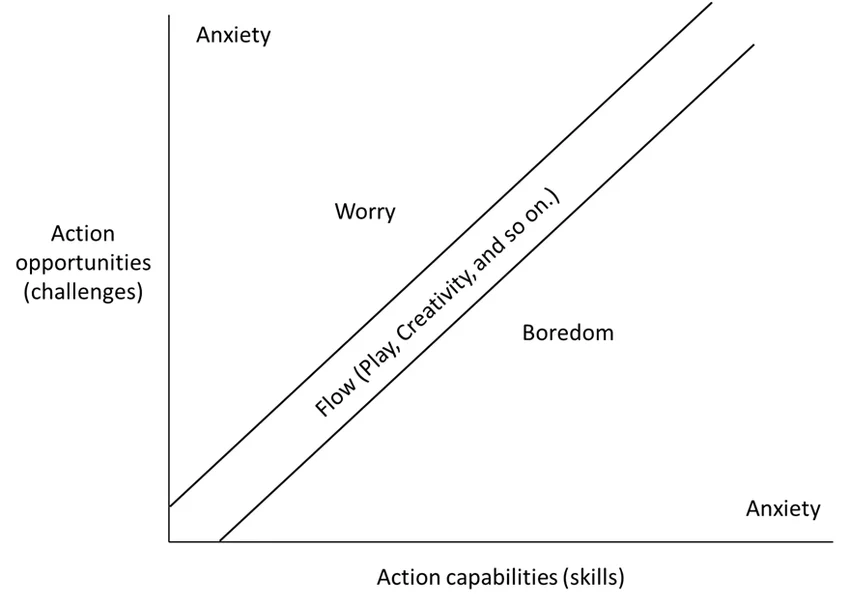
\includegraphics[width=0.72\textwidth]{flowChallenge.png}
    \caption{Challenge-skill model of flow: flow emerges when perceived challenge and perceived skill are balanced at a high level (adapted from \url{https://www.researchgate.net/figure/The-flow-channel-model-adapted-from-Csikszentmihalyi-1975_fig1_259998152}).}
    \label{fig:challengeSkillDiagram}
\end{figure}

\paragraph{Critical Analysis and Limitations of Flow Theory.}
Despite its broad adoption, flow theory has important theoretical and methodological limitations:
\begin{itemize}
    \item \textbf{Subjectivity and the measurement paradox:} Flow is commonly measured via retrospective self-reports. However, because flow involves reduced self-reflection during task execution, attempts to assess it in real time via self reports may disrupt the state itself \autocite{9296229}.
    \item \textbf{Potential maladaptive outcomes:} Although frequently framed as beneficial, prolonged flow in gaming can be linked to problematic patterns such as excessive play, social withdrawal, and neglect of basic needs (e.g., sleep and nutrition) \autocite{harris2023systematic}.
\item \textbf{Model simplification:} The linear challenge-skill representation may underdescribe competitive e-sports settings, where social pressure, team coordination, and situational volatility also shape the experience \autocite{poulus2021determinants}.\end{itemize}

\subsection{Physiological Correlates of Flow}
To complement subjective self-reports, this thesis utilizes physiological measures as objective indicators of the user's state. Other biological markers, such as cortisol, were explicitly excluded from the real-time runtime loop of the proposed prototype. While early neurophysiological studies suggested an inverted U-shaped pattern between cortisol release and flow components, its coarse temporal resolution makes it structurally unsuited for millisecond-level, closed-loop physio-adaptive interventions, which require immediate data streams.

The primary neurophysiological signals considered during model development and context mapping are:

\begin{enumerate}
    \item \textbf{Electrocardiography (ECG):} ECG records the raw electrical activity of the heart, from which \textbf{Heart Rate Variability (HRV)} is derived. While standard stress states are characterized by a purely sympathetic "fight-or-flight" response, recent literature indicates that the flow experience is uniquely characterized by a complex \textbf{dual-branch co-activation} pattern of both the sympathetic and parasympathetic nervous systems \autocite{uechtritz2026neurophysiological}. This co-activation functions as an index of maximum physiological flexibility, enabling adaptive, high-speed responses to shifting game demands while maintaining a calm cognitive baseline. Tracking HRV parameters thus provides a non-invasive, temporally sensitive method to differentiate the high-arousal engagement of flow from the erratic responses associated with performance anxiety or competitive \enquote{tilt} \autocite{irshad2023wearable}.
    
    \item \textbf{Electroencephalography (EEG):} EEG captures bioelectrical brain activity and serves as a high-resolution indicator of central nervous system (CNS) dynamics. Rather than relying solely on the classic \textit{Transient Hypofrontality Hypothesis}—which posits a temporary down-regulation of conscious processing \autocite{dietrich2004neurocognitive}—the high-tempo demands of competitive e-sports are better mapped through modern frameworks like \textit{Synchronization Theory}, which views flow as an energetic optimization arising from the tight harmonization of attentional and reward networks \autocite{uechtritz2026neurophysiological}. Electrophysiologically, these combined dynamics are marked by increased frontal \textbf{theta oscillations} (indexing intense task-focus) and increased frontocentral \textbf{alpha power} (indexing sensory gating and the suppression of external distractions) \autocite{katahira2018eeg}.

    \item \textbf{Electrodermal Activity (EDA):} EDA measures skin conductance and serves as a direct index of sympathetic nervous system arousal. Its relation to flow is defined by the intensity of engagement along the classic challenge-skill model. While low EDA signaling indicates an under-aroused state of \textbf{boredom}, flow is sustained by moderate-to-high sympathetic tone. Crucially, EDA provides a secondary classification axis to separate flow from anxiety; whereas anxiety yields chaotic, high-amplitude sympathetic spikes, flow exhibits stable, task-aligned, and highly regular arousal dynamics \autocite{irshad2023wearable}.
\end{enumerate}

In addition to internal physiological features, this thesis incorporates \textbf{webcam-based face and head activity tracking} as a primary external behavioral data source. Recent advances in affective computing demonstrate that camera-based sensing holds significant predictive value for non-obtrusive flow detection, mitigating the physical discomfort and motion artifacts frequently induced by heavy skin-contact wearables during intense gaming \autocite{uechtritz2026neurophysiological}. Webcam video feeds capture micro-expressions, facial affect metrics, and structural variables (such as head orientation and fixation metrics) that display distinct negative correlations during flow disruptions or cognitive overloading \autocite{kutt2022biraffe2}.

In the final live deployment phase of this thesis, this multimodal synthesis is structurally restricted: the system isolates and evaluates only the features reproducible by the target prototype hardware—namely \textbf{ECG-derived HRV features from a non-intrusive chest belt } and \textbf{webcam-based affect/behavioral features}. High-density central modalities like EEG and raw EDA are leveraged solely within the secondary dataset feature space during offline training to optimize model convergence boundaries, establishing a scalable and non-obtrusive architecture tailored for high-stakes competitive esports environments.

\subsection{Physio-Adaptive Systems and the Biocybernetic Architecture}
An adaptive system is defined by its ability to modify its behavior, interface, or functionality in response to changing user requirements or environmental contexts \autocite{oppermann1994adaptivity}. A \textbf{physio-adaptive system} represents a specialized sub-class of these systems that utilizes real-time physiological or behavioral signals (e.g., ECG, EEG, EDA, or webcam-based affect features) as control input for its adaptation decisions \autocite{fairclough2009fundamentals}.

\subsubsection{Functional Architecture: The Biocybernetic Loop}
The operational framework of a physio-adaptive system can be grounded as a \textbf{biocybernetic control loop} \autocite{pope1995biocybernetic}. In general terms, this architecture describes a closed feedback cycle between a human user and a computational system. The system continuously senses user-related signals, interprets these signals as indicators of an internal or task-relevant state, and adapts the environment or interface accordingly. The user's response to this adaptation then becomes part of the next sensing cycle. As illustrated in Figure~\ref{fig:biocyberneticLoop}, the loop therefore provides a general structure for closed-loop human-computer interaction rather than a flow-specific model only.

\begin{figure}[htbp]
    \centering
    \begin{tikzpicture}[>=stealth, every node/.style={font=\small}]
        \node[draw, rounded corners, align=center, minimum width=3.2cm, minimum height=1.1cm] (sense) at (0,0) {Sensing\\(User Signals)};
        \node[draw, rounded corners, align=center, minimum width=3.2cm, minimum height=1.1cm] (infer) at (5,0) {Interpretation\\(State Inference)};
        \node[draw, rounded corners, align=center, minimum width=3.2cm, minimum height=1.1cm] (adapt) at (10,0) {Adaptation\\(System Output)};
        \node[draw, rounded corners, align=center, minimum width=3.8cm, minimum height=1.1cm] (user) at (5,-2.3) {User\\(Cognitive \& Affective State)};

        \draw[->, thick] (sense) -- node[above] {Features} (infer);
        \draw[->, thick] (infer) -- node[above] {Decision} (adapt);
        \draw[->, thick] (adapt) -- node[right] {Intervention} (user);
        \draw[->, thick] (user) -- node[left] {Response} (sense);
    \end{tikzpicture}
    \caption{General biocybernetic control loop used in physio-adaptive systems. The system senses user-related signals, infers a latent state, adapts the environment, and observes the user's response (adapted from \textcite{chiossi2023how}).}
    \label{fig:biocyberneticLoop}
\end{figure} 

The loop consists of three primary stages:
\begin{itemize}
    \item \textbf{Sensing (Input):} Continuous acquisition of user-related signals, such as physiological, behavioral, or contextual data.
    \item \textbf{Interpretation (Inference):} Transformation of these signals into features and inference of a latent user state or task-relevant condition.
    \item \textbf{Adaptation (Output):} Execution of a system response intended to support the user, stabilize performance, or reduce disruptive conditions.
\end{itemize}

In this thesis, the general loop is specified for flow support in competitive e-sports. During model development, sensing includes physiological signals such as ECG, EEG, and EDA, while the live evaluation focuses on ECG-derived HRV features and webcam-based affect features. In the interpretation stage, machine learning models map these features to \enquote{flow} or \enquote{non-flow} labels, following prior work on HRV-based flow classification \autocite{9296229}. In the adaptation stage, the system uses the inferred flow state to decide whether environmental interventions, such as shielding distracting notifications, should be triggered.

\subsubsection{Application in E-Sports: Shielding and the Measurement Paradox}
While office-based physio-adaptive designs often implement shielding mechanisms to suppress digital notifications \autocite{ubt_eref88160}, the application in competitive e-sports requires more domain-specific interventions. For instance, recent research in LoL has explored providing real-time data visualizations to support player training and performance monitoring \autocite{10.1145/3549506}. The necessity for such automated, non-intrusive interventions is driven by the inherent \enquote{obtrusiveness} of traditional measurement—whereby manual self-reporting would inevitably disrupt the very flow state the system is intended to protect. By integrating these measures directly into the gaming environment, the system maintains the player's immersion while providing actionable feedback or mitigating external distractions.

Because flow involves a recession of self-referential thought, mid-task surveys create a methodological paradox: the act of measuring the state requires the player to self-reflect, which inherently disrupts or terminates the flow experience \autocite{9296229, Moneta2012}. By utilizing the biocybernetic loop to provide \enquote{biologically transparent} monitoring, physio-adaptive systems can protect the user's immersion without the need for intrusive queries, mitigating the risk of distractions that can otherwise take a user up to 23 minutes to recover from \autocite{ubt_eref88160}.

\subsubsection{General Limitations of Physio-Adaptive Flow Support}
Although physio-adaptive systems offer a promising way to support flow without interruptive self-reports, their use also introduces methodological, technical, and contextual limitations. These limitations concern both existing NeuroIS approaches such as FlowShield and the specific transfer of such ideas to LoL.

\paragraph{Limitations of the FlowShield approach by Adam et al.}
The work by \textcite{ubt_eref88160} provides an important precedent for neuro-adaptive flow support and intelligent interruption management. However, its evaluation context differs substantially from competitive e-sports. The field evaluation demonstrates ecological relevance for knowledge-work settings, but it does not establish that the same intervention logic transfers directly to time-critical team games. In office work, notifications can often be delayed without immediate collective consequences; in LoL, however, communication may be strategically relevant within seconds. In addition, the FlowShield approach focuses on IT-mediated interruptions and flow support in work tasks, whereas e-sports involve rapid motor input, voice communication, emotional arousal, and volatile game states. Consequently, Adam et al.'s results should be treated as design guidance rather than direct evidence that autonomous shielding is suitable for competitive gaming. Their own discussion of limitations and future research also implies the need for further validation across contexts, longer-term use, and more diverse real-world settings \autocite{ubt_eref88160}.

\paragraph{Limitations in the LoL context.}
\begin{itemize}
    \item \textbf{Signal Ambiguity During Gameplay:} In LoL, physiological changes are not caused by cognitive flow alone. Team fights, rapid mouse and keyboard actions, voice-chat pressure, caffeine intake, and emotional reactions to deaths or objective losses can all alter ECG-derived HRV or facial affect. This creates a risk of false positives, where stress, physical activation, or frustration is misclassified as flow \autocite{fairclough2009fundamentals}.
    \item \textbf{Context Sensitivity of Interventions:} Autonomous adaptations can be problematic in LoL because the relevance of an interruption depends strongly on match context. A notification or Discord message may be irrelevant during farming but important during champion select, pauses, scrims, or team coordination. If the system suppresses information at the wrong moment, it may create \enquote{automation surprise} and reduce the player's perceived control \autocite{ubt_eref88160}.
    \item \textbf{Webcam and Environment Constraints:} Webcam-based affect recognition is sensitive to lighting, camera angle, occlusions from headsets or hands, and limited facial movement during intense concentration. In LoL, players may also look away from the camera toward secondary monitors or teammates, which can reduce the reliability of webcam-derived features.
    \item \textbf{Privacy and Competitive Integrity:} Continuous ECG and webcam monitoring may reveal sensitive information about stress, emotion, or performance pressure. In competitive LoL environments, such data require strict privacy protection and must be handled carefully so that monitoring does not conflict with player autonomy, team confidentiality, or tournament integrity \autocite{fairclough2009fundamentals}.
\end{itemize}


    \clearpage  
    \section{Method}
        
\noindent
This chapter details the methodological framework employed to investigate physio-adaptive flow detection. Following a \textbf{mixed-method design} \autocite{creswell2017research}, integrates qualitative insights from semi-structured interviews with athletes and industry experts with the technical implementation with the technical implementation of a computational model. In a sequential triangulation design, the methods are not conducted in isolation; rather, the output of the qualitative strand (Phase 1) serves as the foundational input for the development of the technical solution (Phase 2), which is then validated through user-centric testing (Phase 3). This approach ensures that the resulting machine learning (ML) models are not only technically accurate but are built upon the \enquote{ground truth} of the lived experiences of e-sports practitioners. The study follows a three-phase progression, moving from theoretical discovery to practical application and final assessment. As illustrated in Figure~\ref{fig:sequentialTriangulation}, the findings from the initial requirement definition inform the implementation of the problem solution, which is subsequently integrated during the final evaluation.

\begin{figure}[htbp]
    \centering
    \begin{tikzpicture}[>=stealth, every node/.style={font=\small}]
        \node[draw, rounded corners, minimum width=4.2cm, minimum height=1.1cm, align=center] (qual) at (0,0) {Phase 1:\\Requirement Definition\\(Interviews, GTM Coding)};
        \node[draw, rounded corners, minimum width=4.2cm, minimum height=1.1cm, align=center] (quan) at (5.8,0) {Phase 2:\\Implementation\\(Problem Solution)};
        \node[draw, rounded corners, minimum width=4.4cm, minimum height=1.1cm, align=center] (intg) at (11.8,0) {Phase 3:\\Evaluation\\(Triangulated Validation)};

        \draw[->, thick] (qual) -- node[above] {Design Specs} (quan);
        \draw[->, thick] (quan) -- node[above] {Artifact} (intg);
        \draw[->, dashed, thick, bend left=18] (qual.north) to node[above] {Requirement Check} (intg.north);
    \end{tikzpicture}
    \caption{Sequential triangulation design used in this study: requirement definition, implementation/problem solution, and evaluation.}
    \label{fig:sequentialTriangulation}
\end{figure}

The phases are defined as follows:

\begin{enumerate}
    \item \textbf{Phase 1: Requirement Definition (Qualitative Discovery):} Through semi-structured interviews and a review of the literature, the specific triggers and inhibitors of flow in e-sports are identified. This phase uses Grounded Theory Methodology (GTM) to analyze the data, providing the specific functional requirements for a Physio-Adaptive system \autocite{recker2021researchmethods}.
    
    \item \textbf{Phase 2: Implementation (Problem Solution):} In this phase, the physio-adaptive prototype is developed to address the requirements identified in Phase 1. This involves building the machine learning pipeline (using secondary datasets) and the adaptation layer. The focus here is on the technical creation of a solution that can maintain the flow of the athletes.
    
    \item \textbf{Phase 3: Evaluation (Qualitative Validation):} The completed system is assessed via user testing and a second round of interviews. This final step compares the system's objective classification performance against the user's subjective experience. The goal is to determine if the implemented solution actually meets the requirements defined in the initial qualitative phase.
\end{enumerate}

\subsection{Requirement definition: Semi-Structured Interviews}



\subsubsection{Sampling and Participant Recruitment}
To ensure a focused analysis of flow support in a realistic competitive setting, this study uses a purposive, stratified sampling strategy focused on the LoL competitive ecosystem and on expert knowledge relevant to game-adjacent adaptation. The resulting requirements are \textbf{not} treated as universally valid for all e-sports players. Instead, they are interpreted as design-oriented requirements for a physio-adaptive prototype in the context of competitive LoL.

To establish a triangulated requirements baseline, the qualitative sample consists of three complementary cohorts and a total of nine semi-structured interviews ($N = 9$):
\begin{enumerate}
    \item \textbf{Competitive active players ($n = 3$):} Players provide first-hand accounts of gameplay flow, stress, interruptions, and competitive routines.
    \item \textbf{Game design experts ($n = 3$):} Experts assess whether the proposed adaptive measures are compatible with game mechanics, interface design, pacing, player agency, and competitive integrity.
    \item \textbf{Physiological computing experts ($n = 3$):} Experts assess the technical and methodological plausibility of sensor fusion, real-time data processing, and biocybernetic feedback loops.
\end{enumerate}

The primary player target group is defined as \textbf{Tier 2: high-ELO and semi-professional players}. This group is selected because it combines high competitive pressure and advanced game knowledge with more realistic accessibility for interviews and prototype testing than fully professional Tier 1 players. 

\begin{itemize}
    \item \textbf{Target Player Groups and Stratification:} Participants are categorized into three distinct tiers based on their standing within the official LoL competitive ladder, which comprises the ranks of \textit{Iron, Bronze, Silver, Gold, Platinum, Emerald, Diamond, Master, Grandmaster,} and \textit{Challenger} \autocite{gong2020league}. The stratification is not intended to give all tiers equal authority over the final requirements. Instead, requirements are weighted according to their relevance for the Tier 2 target context:
    \begin{enumerate}
        \item \textbf{Professional Athletes (Tier 1):} Competitors currently active in premier professional leagues such as the \textit{LEC} (EMEA), \textit{LCS} (North America), or the \textit{Prime League Pro Division} (DACH). While players in this tier are almost exclusively ranked in \textit{Challenger}, they are defined by their professional status and contractual obligations. Tier 1 perspectives are used only for contextual orientation where available, but Tier 1 requirements are not inferred from lower-tier participants. \textit{Note: Recruiting within this tier represents a significant methodological challenge due to restricted schedules and strict contracts.}
        
        \item \textbf{High-ELO / Semi-Professional Players (Tier 2):} Highly skilled individuals positioned at the apex of the regional ladder. This group encompasses players in the \textbf{Diamond, Master, Grandmaster,} and \textbf{Challenger} tiers who are not currently active in Tier 1 leagues. These ranks represent the primary target population of the thesis, where the demand for flow-maintenance and the cost of interruptions are expected to be high while access for empirical work remains feasible \autocite{gong2020league}.
        
        \item \textbf{Casual and Intermediate Gamers (Tier 3):} Enthusiasts playing for recreation or amateur-level competition. This group covers the vast majority of the player distribution and includes all individuals ranked from \textbf{Iron, Bronze, Silver, Gold, Platinum,} through to \textbf{Emerald} \autocite{gong2020league}. Tier 3 participants are not used to infer the needs of Tier 1 or Tier 2 players. Their role is strictly to reveal accessibility issues, general usability expectations, and contrasts between casual and advanced competitive play.
    \end{enumerate}

    \item \textbf{Selection Criteria:} Inclusion and exclusion criteria are defined separately for each cohort to make participant selection transparent and comparable across groups:
    \begin{itemize}
        \item \textbf{Competitive Active Players:} Players are included if they are at least 18 years old, actively play LoL, can provide a verifiable \textit{Riot ID} or \textit{Summoner Name}, and currently meet the Tier 2 rank definition. They must also be willing to discuss their competitive setup, communication practices, interruption experiences, and willingness to use an ECG chest belt and webcam in a later prototype evaluation. Players are excluded if their rank cannot be verified, if they are below Diamond at the time of recruitment, if contractual obligations prevent open participation, or if they do not provide informed consent.
        \item \textbf{Game Design Experts:} Game design experts are included if they have worked in game design research or the game industry for at least three years. Eligible experts must have practical or scholarly experience with the design of computer games, including published games, prototypes, research artifacts, or equivalent interactive game projects. The search strategy prioritizes experts who have worked on LoL or comparable multiplayer online battle arena (MOBA) games, because this experience is most relevant for assessing intervention timing, player agency, interface constraints, and competitive integrity. Experts are excluded if their experience is limited to casual game use, if they cannot substantiate relevant game design experience, or if they lack direct professional or scholarly exposure to game mechanics, interface design, or player experience.
        \item \textbf{Physiological Computing Experts:} Physiological computing experts are included if they have worked in physiological computing research or industry for at least three years. Eligible experts must have experience with physiological sensing methods, data acquisition, signal processing, and data-processing workflows, including machine learning pipelines. The search strategy prioritizes experts with experience in ECG or webcam-based measurements, ideally in gaming, entertainment computing, HCI, or other interactive real-time applications. Experts are excluded if their expertise is unrelated to physiological sensing, data acquisition, signal processing, machine learning-based analysis, or human-centered adaptive systems, or if they cannot assess the ethical and practical implications of using physiological signals in an adaptive system.
    \end{itemize}

    \item \textbf{Hardware and Software Context:} Interviews document each participant's relevant setup or professional frame of reference, including computer performance level, monitor configuration, input devices, headset and voice communication setup, operating system environment, and familiarity with ECG or webcam-based sensing. This information is treated as contextual data rather than as a universal technical standard. The prototype is therefore designed for the Tier 2 context and common high-performance gaming setups, not as a guaranteed fit for all professional tournament infrastructures or casual home environments.

    \item \textbf{Recruitment Channels:} Player participants are recruited through university e-sports structures, especially \textit{Uni-Liga} teams at the University of Duisburg-Essen, supplemented by high-ELO community structures such as competitive \textit{Discord} servers and public LoL player forums. Game design experts are contacted through university game design programs, academic faculties at partner art/design universities, professional game development networks, LinkedIn, studio contact pages, and game development directories. Physiological computing experts are contacted through the University of Duisburg-Essen's Entertainment Computing and HCI chairs, research lab websites, publication-based email outreach, and professional networks related to physiological sensing and interactive systems.

    \item \textbf{Verification Procedure:} Player eligibility is verified through the provided \textit{Riot ID} or \textit{Summoner Name} and public ranking or match-history information. Expert eligibility is verified through public institutional profiles, professional profiles, publication records, industry credentials, or self-reported career histories checked for consistency with the inclusion criteria. All participants must provide informed consent before the interview.
\end{itemize}



\subsubsection{Data Collection and Tooling}
Interviews are conducted as semi-structured sessions to allow for emergent themes while ensuring core research questions are addressed. 

\begin{itemize}
    \item \textbf{Interview Platform:} Remote interviews are conducted via \textit{Microsoft Teams} or \textit{Zoom}, utilizing their built-in high-fidelity audio recording features.
    \item \textbf{Transcription:} Initial transcription is performed using \textit{f4transcript}. This software is utilized because it ensures that all data processing and storage occur exclusively on servers located in Germany, adhering to the highest standards of the Federal Data Protection Act (BDSG) and GDPR.
\end{itemize}

\subsubsection{Data Privacy and Ethical Considerations}
In accordance with the General Data Protection Regulation (GDPR), strict privacy standards are maintained throughout the research lifecycle:

\begin{itemize}
    \item \textbf{Informed Consent:} Before the interview, all participants must sign a digital consent form detailing the study's purpose, the nature of data collection, and their right to withdraw at any time without penalty.
    \item \textbf{Data Storage and Security:} All raw audio recordings and transcripts are stored on encrypted, password-protected servers provided by the university. Access is strictly limited to the primary researcher.
    \item \textbf{Anonymization:} Data is pseudonymized immediately following the transcription phase. Real names and identifying details are replaced with alphanumeric codes (e.g., P1-Elite, P2-Casual) to ensure participant privacy during the Grounded Theory analysis.
    \item \textbf{Third-Party Processing:} For automated transcription (Otter.ai), data is uploaded to secure, SOC 2 Type II compliant servers and is permanently deleted from the cloud service once the manual verification phase is complete.
\end{itemize}

\subsubsection{Qualitative Analysis: GTM Coding Workflow}
Following the methodology described by \textcite{recker2021researchmethods}, the analysis utilizes a systematic coding workflow. This process is managed using \textit{MAXQDA} \autocite{MAXQDA2022}, a professional Computer-Assisted Qualitative Data Analysis Software (CAQDAS). 

As a focused application of Grounded Theory Methodology (GTM), this thesis emphasizes coding-based analysis rather than full theory generation. Interview data are iteratively processed through open, axial, and selective coding to derive practically relevant categories for physio-adaptive system design \autocite{recker2021researchmethods,delveholempaecher2024openaxialselective}. In this workflow, open codes are first grouped into higher-order relationships during axial coding (Figure~\ref{fig:axial_coding}), and these relationships are then consolidated into a central explanatory category during selective coding (Figure~\ref{fig:selective_coding}).

The software facilitates the iterative transition between data collection and analysis, allowing for the organized management of \textit{Open}, \textit{Axial}, and \textit{Selective} codes. By utilizing MAXQDA's creative coding and visual mapping tools, the researcher can more effectively identify the "Core Category" that defines the e-sports flow experience, ensuring a rigorous application of the GTM procedures as outlined by \textcite{recker2021researchmethods}.

\begin{figure}[H]
    \centering
    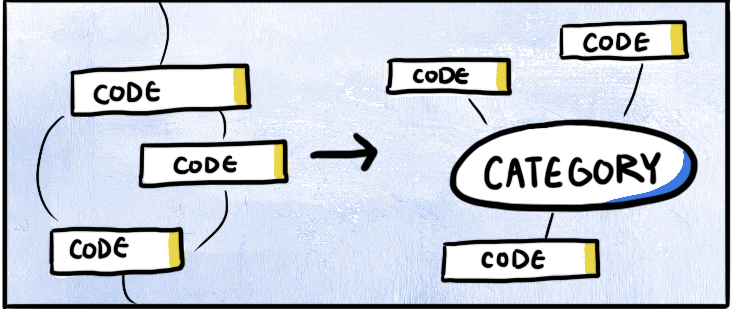
\includegraphics[width=0.9\textwidth]{AxialCoding_DelveTool_2.png}
    \caption{Example of creating axial codes from open codes (Source: \autocite{delveholempaecher2024openaxialselective}).}
    \label{fig:axial_coding}
\end{figure}

\begin{figure}[htbp]
    \centering
    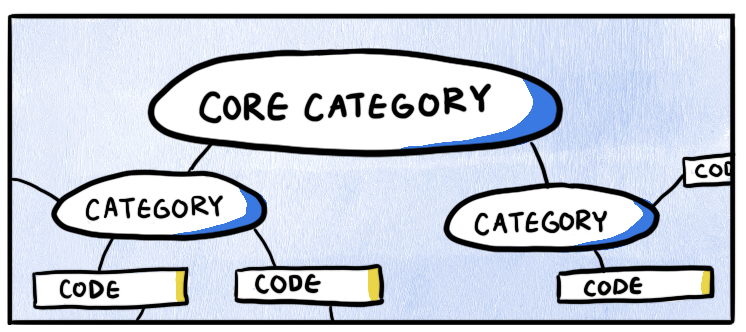
\includegraphics[width=0.9\textwidth]{SelectiveCoding_DelveTool.png}
    \caption{Example of creating selective code from axial codes (Source: \autocite{delveholempaecher2024openaxialselective}).}
    \label{fig:selective_coding}
\end{figure}


\begin{itemize}
    \item \textbf{Open Coding:} Transcripts are broken down into discrete "incidents." Codes such as "Environmental Distraction," "Cognitive Tunneling," and "Post-interruption Frustration" are assigned.
    \item \textbf{Axial Coding:} Concepts are reassembled to identify relationships. For example, the code "Digital Pings" may be linked as a causal condition to the category "Flow Breakage."
    \item \textbf{Selective Coding:} A central core category, such as \enquote{User-Centric Requirements for Physio-Adaptive Flow Support,} is identified. This category integrates the previously identified inhibitors and facilitators to explain the overarching conditions under which an e-sports athlete accepts or rejects autonomous system interventions. By centering the analysis on these requirements, the qualitative strand provides a direct blueprint for the technical implementation in the subsequent phase.
\end{itemize}

\subsection{Implemention: Computational Experimentation}

\subsubsection{Secondary Data Sources}
Rather than collecting primary physiological data for model training, this thesis conducts a secondary analysis of two labeled physiological datasets. The datasets were selected because they serve complementary roles in the model-development strategy: BIRAFFE2 provides the gaming-oriented basis for multimodal state detection, whereas the Irshad et al. / PhySF dataset offers an additional flow-specific physiological reference dataset. To make the two sources comparable, the shared training space is restricted to the physiological modalities available in both datasets, namely \textbf{EEG, ECG, and EDA}. Webcam-based facial data is considered only in BIRAFFE2-derived models, because the Irshad et al. dataset does not include webcam images or facial video recordings.
\begin{enumerate}
    \item \textbf{BIRAFFE2 Dataset \autocite{kutt2022biraffe2}:}
    \begin{itemize}
        \item \textbf{Selection Rationale:} BIRAFFE2 was selected because it captures affective responses in a gaming context and therefore provides high relevance for the gaming-oriented model-development track. Its main advantage is its \textbf{multimodal scope}: physiological signals are synchronized with gamepad telemetry and \textbf{video-based facial expressions}. This makes it possible to examine internal physiological patterns alongside external behavioral and visual indicators of player state.

        \item \textbf{Dataset Context and Available Modalities:} Participants completed affective gaming tasks, such as a \textit{Space Invaders} clone, while multiple synchronized data streams were recorded. The available BIRAFFE2 data includes physiological signals (\textbf{EEG, ECG, and EDA}), visual and behavioral data (\textbf{webcam-based facial recordings/photos} and \textbf{full gameplay screencasts}), and physical interaction metrics (\textbf{gamepad telemetry}).

        In the comparative model-development strategy, BIRAFFE2 is treated as the basic dataset because it contains both the shared physiological modalities and the additional webcam-based facial data. The BIRAFFE2-derived models therefore define the full multimodal benchmark as well as the ECG--webcam deployment-oriented prototype path. For cross-dataset comparison, however, the physiological feature space remains limited to \textbf{EEG, ECG, and EDA}, since these modalities also exist in the Irshad et al. / PhySF dataset.

        \item \textbf{Ground Truth Strategy:} The primary ground truth is derived from the \textbf{GEQ Core Module} \autocite{ijsselsteijn2013game}, a standardized instrument for evaluating game experience across seven components. For flow-state labeling, this thesis uses the \textbf{Flow subscale}, which consists of five items:
        \begin{enumerate}
            \item Item 3: \enquote{I forgot everything around me.}
            \item Item 12: \enquote{I was fully occupied with the game.}
            \item Item 18: \enquote{I lost track of time.}
            \item Item 25: \enquote{I felt completely absorbed.}
            \item Item 33: \enquote{I was deeply concentrated in the game.}
        \end{enumerate}
        Each item is rated on a 5-point Likert scale (0 = \textit{not at all} to 4 = \textit{extremely}). The flow label is generated by calculating the mean score across these items. High-fidelity flow states are identified when this mean exceeds a defined threshold (e.g., $>3.0$), enabling a direct mapping between physiological patterns and the subjective dimensions of immersion, absorption, and concentration.
    \end{itemize}

    \item \textbf{Irshad et al. Dataset \autocite{irshad2023wearable}:}
    \begin{itemize}
        \item \textbf{Selection Rationale:} The Irshad et al. / PhySF dataset was selected because it was specifically curated for flow recognition with consumer-grade and research-grade wearable sensors. It therefore complements BIRAFFE2 by providing a flow-focused physiological benchmark and by reflecting the type of non-invasive sensing that is relevant for home, training, or facility-based e-sports settings.

        \item \textbf{Dataset Context and Available Modalities:} The PhySF dataset used by Irshad et al. was collected during work-related tasks and is used for binary flow recognition rather than for modeling boredom, flow, and stress as three separate target states. Participants first completed a baseline recording and then performed mathematical and reading tasks while multimodal physiological signals were recorded. The dataset combines three hardware devices: an \textbf{EMOTIV Insight} headset for EEG, an \textbf{Empatica} wristband for PPG, infrared thermopile skin temperature, and EDA, and a \textbf{Biosignalsplux RespiBAN} chest wearable for respiration, EOG, ECG, and EMG \autocite{irshad2023wearable}. Importantly, this dataset does \textbf{not} contain webcam images or facial video data; it contributes strictly wearable physiological signals to this thesis \autocite{irshad2023wearable}.
        
        \item \textbf{Ground Truth Strategy:} The ground truth in the Irshad et al. dataset is not based on the \textit{Flow Short Scale (FSS)} and is not collected through continuous in-task self-reporting, because such interruptions would disturb the target state. Instead, task recordings are retrospectively segmented using participants' post-task self-reports. After each task, participants indicated whether they had experienced flow and, if so, in which third of the task the flow episode occurred \autocite{irshad2023wearable}. Physiological windows from the reported flow interval are labeled as \textit{flow}, whereas the remaining task windows and recordings without reported flow are labeled as \textit{non-flow}. This produces temporally localized binary labels for flow/no-flow classification rather than continuous questionnaire scores \autocite{irshad2023wearable}.
    \end{itemize}
\end{enumerate}


\noindent
Based on this modality overlap, four model combinations are trained and compared:
\begin{enumerate}
    \item \textbf{BIRAFFE2 full multimodal model:} EEG, ECG, EDA, and webcam-based facial data.
    \item \textbf{Irshad/PhySF full physiological model:} EEG, ECG, and EDA without webcam data, because the dataset contains no webcam images.
    \item \textbf{BIRAFFE2 deployment-oriented model:} ECG and webcam-based facial data, matching the planned live prototype hardware.
    \item \textbf{Irshad/PhySF deployment-oriented baseline:} ECG-only physiological features, because the dataset has ECG but no webcam data.
\end{enumerate}
This structure preserves the available modality descriptions of each dataset while making clear which features are actually used for model training and which model paths are dataset-specific.

\subsubsection{The Machine Learning Pipeline}
The development and optimization of the supervised learning pipeline are implemented in \textit{Python 3.9}. This specific version was selected to ensure a stable execution environment with broad compatibility for the complex dependency trees of high-level physiological libraries, avoiding the experimental instability of newer releases while maintaining support for modern asynchronous processing.

The model-development process explicitly distinguishes between dataset-specific full and deployment-oriented configurations to separate offline benchmarking from practical runtime capabilities. The full benchmark tracks use the overlapping physiological modalities \textbf{EEG, ECG, and EDA} in both datasets; webcam-based affect features are added only for BIRAFFE2. The deployment-oriented tracks use the signals that can inform the planned prototype path: \textbf{ECG + webcam} for BIRAFFE2 and \textbf{ECG only} for Irshad/PhySF. Additional modalities available in the source datasets (e.g., gamepad telemetry in BIRAFFE2; Respiration, EOG, and EMG in the Irshad dataset) are excluded because they are either structurally incompatible with LoL's mouse-and-keyboard setting or highly susceptible to movement and voice-chat artifacts in e-sports.

Figure~\ref{fig:classification_pipeline} summarizes the complete classification workflow from the two secondary datasets to real-time flow/non-flow prediction. It makes the dataset-specific deployment paths explicit: BIRAFFE2 can feed the ECG--webcam prototype model, whereas the Irshad et al. / PhySF dataset can only feed an ECG-only deployment baseline because it contains no webcam recordings.

\begin{figure}[htbp]
    \centering
    \resizebox{0.96\linewidth}{0.68\textheight}{%
    \begin{tikzpicture}[
        >=stealth,
        % Global node distances (vertical and horizontal)
        node distance=1.25cm and 1.55cm, 
        every node/.style={font=\scriptsize},
        process/.style={draw, rounded corners, align=center, text width=3.15cm, minimum height=1.15cm, inner sep=5pt},
        decision/.style={draw, rounded corners, align=center, text width=3.35cm, minimum height=1.15cm, inner sep=5pt, fill=gray!10},
        dataset/.style={draw, rounded corners, align=center, text width=3.35cm, minimum height=1.15cm, inner sep=5pt, fill=gray!5},
        model/.style={draw, rounded corners, align=center, text width=3.65cm, minimum height=1.3cm, inner sep=5pt, fill=gray!5}
    ]
        % --- ROW 1 (Forward Path) ---
        \node[process] (raw) {Raw Dataset\\Signals};
        \node[dataset, right=of raw] (biraffe) {BIRAFFE2\\ECG, EEG, EDA, Webcam};
        \node[process, right=of biraffe] (prep) {Preprocessing\\Artifact Removal};
        \node[process, right=of prep] (window) {Windowing\\60 s Window / 30 s Step};

        % --- ROW 2 ---
        % Placed directly below BIRAFFE2
        \node[dataset, below=of biraffe] (irshad) {Irshad/PhySF\\Wearables, No Webcam};

        % --- ROW 3 (Return Path) ---
        % Dropped 2.5cm below Windowing to ensure it clears the Irshad node
        \node[process, below=2.5cm of window] (features) {Feature Extraction\\Dataset-Specific Modalities};
        \node[decision, left=of features] (tracks) {Two Feature Tracks\\Full vs. Deployment-Aligned};
        \node[process, left=of tracks] (training) {Model Training\\and Validation};

        % --- ROW 4 (Deployment Path) ---
        % Selection drops below Training, continuing the flow
        \node[process, below=of training] (selection) {Model Selection\\Accuracy, F1, Latency};
        \node[model, right=of selection] (deploy_b) {BIRAFFE2 Prototype Model\\ECG + Webcam Only};
        \node[process, right=of deploy_b] (prediction) {Real-Time Prediction\\Flow / Non-Flow};

        % --- ROW 5 ---
        \node[model, below=of deploy_b] (deploy_i) {Irshad Deployment Baseline\\ECG Only};

        % --- EDGES ---
        % Forward flow
        \draw[->, thick] (raw) -- (biraffe);
        \draw[->, thick] (raw) |- (irshad);
        \draw[->, thick] (biraffe) -- (prep);
        \draw[->, thick] (irshad) -| (prep);
        \draw[->, thick] (prep) -- (window);
        
        % Return flow (Snake)
        \draw[->, thick] (window) -- (features);
        \draw[->, thick] (features) -- (tracks);
        \draw[->, thick] (tracks) -- (training);
        \draw[->, thick] (training) -- (selection);
        
        % Deployment flow
        \draw[->, thick] (selection.east) -- node[above, font=\tiny, midway] {B2} (deploy_b.west);
        \draw[->, thick] (selection.south) |- node[pos=0.25, right, font=\tiny] {PhySF} (deploy_i.west);
        
        % Prediction flow
        \draw[->, thick] (deploy_b.east) -- (prediction.west);
        % The -| notation draws horizontally then vertically into the bottom of prediction
        \draw[->, thick, dashed] (deploy_i.east) -| (prediction.south);
        
    \end{tikzpicture}
    }
    \caption{Dataset-specific model paths for real-time flow prediction.}
    \label{fig:classification_pipeline}
\end{figure}

\begin{itemize}
\item \textbf{Preprocessing:} Signal cleaning and artifact removal are performed using specialized toolkits to ensure high signal-to-noise ratios. \textit{NeuroKit2} is utilized for ECG and EDA data processing due to its comprehensive suite of built-in filters and peak-detection algorithms designed specifically for bio-signal analysis \autocite{makowski2021neurokit2}. For the EEG data, the \textit{MNE-Python} library is employed; it is widely regarded as the industry standard for electrophysiological data, offering robust methods for Independent Component Analysis (ICA) and automated artifact rejection \autocite{gramfort2013mne}. These tools are essential for removing ocular and muscular artifacts which are particularly prevalent in the high-intensity, active environments characteristic of e-sports.

\pagebreak[3]
\item \textbf{Feature Engineering:} Features are extracted using a fixed \textbf{60-second sliding window} with a \textbf{30-second step size}, resulting in 50\% overlap between consecutive windows. The 60-second window is selected as the primary analysis window because HRV frequency-domain features require a sufficiently long segment to produce stable estimates of LF and HF power, whereas substantially shorter windows would make these measures less reliable. The 30-second step size preserves temporal responsiveness by updating the feature representation twice per minute without discarding the physiological stability gained from the longer window. To avoid data leakage, overlapping windows derived from the same participant recording are never split across training and test sets. Instead, splitting is performed at the participant level during cross-validation, so that all windows from a held-out participant remain exclusively in the test fold. This ensures that the model is evaluated on unseen participants rather than on temporally adjacent windows from the same recording. Table~\ref{tab:feature_mapping} provides a specific overview of the feature sets extracted, explicitly differentiated by their target configuration track.

\begin{table}[!tbp]
    \centering
    \scriptsize
    \caption{Overview of Feature Extraction differentiated by Pipeline Configuration.}
    \renewcommand{\arraystretch}{1.3}
    \begin{tabularx}{\linewidth}{|l|L|L|L|}
        \hline
        \rowcolor{black}
        \textbf{\color{white} Signal Modality} & \textbf{\color{white} Statistical Features} & \textbf{\color{white} Frequency-Domain / Temporal} & \textbf{\color{white} Non-linear Features} \\
        \hline
        \multicolumn{4}{|c|}{\cellcolor{gray!20}\textbf{Deployment-Aligned Configuration (Live Prototype \& Full Multimodal)}} \\
        \hline
        \textbf{ECG (HRV)} & Mean HR, SDNN, RMSSD, pNN50 & LF Power, HF Power, LF/HF Ratio & Sample Entropy (SampEn), Detrended Fluctuation Analysis (DFA) \\
        \hline
        \textbf{Webcam} & Mean and Variance of Emotion Probabilities (Neutral, Happy, Angry); Z-axis Rotation & Eye Fixation Duration Percentage; Micro-Expression Peak Frequencies & Gaze Path Length Complexity; Head Orientation Movement Entropy \\
        \hline
        \multicolumn{4}{|c|}{\cellcolor{gray!20}\textbf{Full Multimodal Configuration Only (Offline Benchmarking)}} \\
        \hline
        \textbf{EEG} & Mean PSD per channel, Band Variance & Theta, Alpha, and Beta Power; Alpha/Theta Ratio & Spectral Entropy, Hurst Exponent \\
        \hline
        \textbf{EDA} & Mean SCL, Max SCR Amplitude, SCR frequency & Power Spectral Density (PSD) of phasic component & Lyapunov Exponent, Signal Complexity \\
        \hline
    \end{tabularx}
    \label{tab:feature_mapping}
\end{table}

The extracted features are categorized into three domains:

\begin{itemize}
    \item \textbf{Statistical Features (Arousal Baseline):} These provide a baseline measure of physiological arousal and capture sudden shifts in engagement. For example, sudden shifts in Mean Heart Rate (ECG) represent acute stress responses to in-game events, while stable Neutral affect probabilities (Webcam) establish an immersion baseline.
    
    \item \textbf{Frequency-Domain / Temporal Features (Balance and Immersion):} For HRV, this includes Low Frequency (LF) power, High Frequency (HF) power, and the LF/HF ratio to capture the complex autonomic dual-branch co-activation patterns that characterize physiological flexibility during flow \autocite{uechtritz2026neurophysiological}. For the full multimodal benchmark, EEG power ratios (Alpha/Theta) are included to characterize the depth of cognitive immersion \autocite{katahira2018eeg}, while EDA contributes frequency-domain descriptors of arousal dynamics. In the final live evaluation, this is restricted to the ECG and Webcam temporal features (e.g., fixation durations).
    
    \item \textbf{Non-linear Features (Signal Complexity):} Measures such as Sample Entropy quantify the complexity and regularity of the signals. In flow states, physiological signals often exhibit more \enquote{efficient} regularity, whereas the chaotic patterns seen in states of high anxiety or \enquote{tilt} result in higher entropy values.
\end{itemize}

   \item \textbf{Classification Models:} The selection of machine learning classifiers is informed by the dual requirements of high accuracy and computational efficiency for real-time applications. Following the technical precedent of \textcite{9296229}, this study adopts a multi-model benchmarking approach. 

Initially, a suite of traditional supervised learning algorithms is employed to establish a performance baseline:
\begin{itemize}
    \item \textbf{Support Vector Machines (SVM):} Utilized for their ability to identify optimal hyperplanes in high-dimensional multimodal spaces. SVMs are particularly effective at handling the margin-based separation between "flow" and "non-flow" when the feature space is extensive.
    \item \textbf{Random Forest (RF) and Gradient Boosting (XGBoost):} These ensemble methods are included as they are robust against outliers and can model non-linear relationships without intensive hyperparameter tuning. Crucially, Random Forest provides \textit{feature importance} rankings, which allow for the interpretability of which specific markers (e.g., HRV time-domain metrics vs. Webcam affect probabilities) are most indicative of flow \autocite{9296229}.
    \item \textbf{k-Nearest Neighbors (k-NN):} A non-parametric baseline used to assess the local cluster density of physiological states in the feature space.
\end{itemize}

To map the complex dynamics of the "Flow Channel," this research additionally evaluates three specific Deep Learning (DL) architectures:

\begin{itemize}
    \item \textbf{Long Short-Term Memory (LSTM):} Selected specifically to address the \textbf{temporal dependency} of flow. Unlike traditional models that treat data windows as independent points, LSTMs utilize a gated memory mechanism to "remember" previous physiological states. An LSTM can detect the \textit{transition} into flow by analyzing the sequence of changes in heart rate variability and emotion probabilities over time.
    
    \item \textbf{Convolutional Neural Networks (CNN):} Chosen for their \textbf{automated feature extraction} capabilities. 1D-CNNs are highly effective at identifying local patterns (morphologies) in raw waveforms. In this thesis, 1D-CNNs are used to detect specific patterns directly in the raw ECG signal from the chest belt without requiring manual derivation of every HRV band.
    
    \item \textbf{Multi-Layer Perceptron (MLP):} Included to model \textbf{non-linear sensor fusion}. The MLP maps the interactions between disparate data sources—for example, evaluating if a specific decrease in heart rate variability interacting with a simultaneous increase in "Neutral" facial affect probabilities outperforms linear baseline models.
\end{itemize}

The final model selection is determined by an empirical comparison of accuracy, F1-score, precision, recall, and \textit{inference latency} across both the full multimodal and deployment-aligned configurations. The full multimodal models provide a comparative benchmark, while the model selected for the prototype must remain compatible with the deployment-aligned ECG--webcam feature space and real-time latency constraints.
\end{itemize}

\subsection{Research Environment: LoL}
To ensure the feasibility of identifying and implementing specific adaptive measures, this study focuses exclusively on the Multiplayer Online Battle Arena (MOBA) title LoL. LoL provides a highly structured competitive environment with distinct gameplay phases that naturally map to the Flow Channel model: the repetitive, skill-dominant \enquote{laning phase} (risk of boredom) and the high-intensity, cognitively demanding \enquote{teamfight} phase (risk of anxiety).

\subsubsection{Data Acquisition: The Riot Games Live Client API}
The primary technical interface for game-state awareness is the \textbf{Riot Games Live Client Data API}. Unlike standard web-based APIs, this interface runs locally on the user's machine, providing real-time JSON-formatted data regarding the active match. This allows the physio-adaptive system to synchronize physiological signals with objective in-game events without violating anti-cheat protocols.

Key data points utilized from the local endpoint (\texttt{https://127.0.0.1:2999/liveclientdata/allgamedata}) include:
\begin{itemize}
    \item \textbf{Player Vitality and Stats:} Real-time monitoring of Health, Mana, and Level to assess current combat pressure.
    \item \textbf{Event Triggers:} Immediate notification of Kills, Deaths, and Objective captures (e.g., Baron or Dragon), which serve as temporal markers for physiological spikes.
    \item \textbf{Game Timing:} Synchronization of the match clock with the sensor timestamps to correlate fixed 60-second feature windows, updated at 30-second intervals, with specific game phases.
\end{itemize}

\subsubsection{Adaptive Measures: Real-Time Cognitive and Tactical Shielding}
Given that the game client itself is a closed system, the \enquote{problem solution} (Phase 2) focuses on adapting the user's immediate interactive ecosystem and peripheral environment to protect the user's flow state from disruption. Moving beyond rudimentary operating-system-level notification suppression---which competitive athletes may already manage manually---the adaptation engine targets context-aware adjustments outside the protected game client, grounded in affective gaming, flow-support, and cognitive-load-oriented interaction design \autocite{ubt_eref88160,9296229,irshad2023wearable}. The following measures are identified as actionable intervention categories for a prototype evaluation:

\begin{enumerate}
    \item \textbf{External Visual Shielding:} Rather than modifying the in-game HUD, the prototype manages only game-external visual stimuli, such as system notifications, companion dashboards, stream overlays, or secondary-monitor content. When the multimodal classifier detects high cognitive load during critical match phases identified through the local game-state data, non-essential external visual elements can be hidden, dimmed, or delayed. This reduces avoidable visual noise while preserving the integrity of the official game client.
    
    \item \textbf{Intelligent Acoustic Partitioning:} To prevent auditory overload without interfering with vital team communication, the prototype can apply operating-system-level audio rules to external applications. When real-time physiological metrics indicate peak cognitive load during combat events, background applications such as music players can be attenuated, while communication channels and in-game audio remain under the player's control. This keeps the intervention technically feasible and avoids altering competitive game information.
    
    \item \textbf{Attentional Peripheral Cues:} A potential inhibitor of sustained flow in competitive environments is stress-induced narrowing of attention. When webcam-based affect probabilities indicate elevated frustration or anxiety in combination with an ECG-derived reduction in predicted flow, the system can trigger subtle ambient cues outside the game client, for example through peripheral lighting or a secondary display. These cues are intended as non-intrusive reminders to reset attention without injecting tactical information into the match.
    
    \item \textbf{Context-Aware Information Gating:} To reduce automation surprise and preserve player agency, the intensity and duration of interventions are gated by real-time match-state data and conservative safety rules. Shielding mechanisms are activated only during clearly defined high-load windows, such as active combat or objective contests, and are scaled back during lower-pressure phases such as respawn periods or post-fight transitions. The player can override or disable the interventions at any time.
\end{enumerate}



\subsection{Implementation of the Physio-Adaptive System for E-Sports}
Following the model-development phase, the implementation of the physio-adaptive system is conceptualized as a real-time pipeline that links physiological sensing, state inference, and intervention logic. The implementation targets competitive e-sports scenarios in which rapid context changes and high cognitive load require low-latency adaptation.

\begin{itemize}
    \item \textbf{Input Layer:} Multimodal data streams—specifically \textbf{ECG-derived HRV metrics} from the chest belt and \textbf{facial affect probabilities} from the webcam—are continuously acquired and segmented into 60-second sliding windows with a 30-second step size for near-real-time analysis. This ensures that the input features remain strictly limited to the data provided by the provided hardware, allowing for seamless transition from training on the filtered dataset to the live prototype evaluation.
    \item \textbf{Inference Layer:} The trained classifier predicts flow versus non-flow states for each window and outputs a confidence score used for decision-making.
    \item \textbf{Adaptation Layer:} This layer serves as the intervention engine, where a rule-based controller translates the machine learning model's state predictions into specific adaptive actions. Crucially, the logic governing this layer is \textbf{directly derived from the qualitative requirements established in the first phase of the Sequential Triangulation}. 

    Through the Grounded Theory Methodology (GTM) analysis of semi-structured interviews, specific \textit{inhibitors} and \textit{facilitators} of flow were identified. These qualitative categories (derived via Open, Axial, and Selective coding) define the parameters of the "intelligent notification handling." For example, the decision of which alerts are classified as "non-urgent" and the specific timing of the "shielding" duration are grounded in the participants' lived experiences of competitive pressure. By mapping the GTM-derived user needs to the Adaptation Layer, the system ensures that the biocybernetic intervention is not only technically triggered but also contextually appropriate for e-sports athletes.
    \item \textbf{Safety and Override Mechanism:} To preserve user agency, the system includes manual override options and configurable thresholds for adaptation intensity.
\end{itemize}

In practical terms, the implementation is treated as a prototype architecture that can be integrated into game-adjacent environments (communication overlays, desktop notification managers, or tournament training setups) rather than as a full production deployment.

\subsection{Evaluation of the Adaptive System}
The evaluation of the developed solution follows a qualitative validation approach designed to assess the practical utility and experiential acceptance of the system. Crucially, the success criteria for the evaluation are \textbf{directly mapped back to the design requirements identified in the first phase}, ensuring that the system's performance is judged against the actual needs of e-sports practitioners.

\subsubsection{Interview-Based Evaluation Process}
To assess the system's effectiveness, a second round of \textbf{semi-structured interviews} is conducted, utilizing a hybrid evaluation approach. In the \textbf{live pilot phase}, participants are actively equipped with the \textbf{ECG chest belt} and monitored via the \textbf{webcam} while playing LoL. This setup allows for the direct observation of the system's real-time adaptive behavior and provides a basis for immediate post-game feedback regarding the accuracy of flow detection and the utility of the interventions.

If both dataset-derived classifiers achieve competitive baseline performance during the preceding model-development phase, the live pilot evaluation uses a \textbf{between-subject model allocation}. One half of the physical pilot participants uses the deployment-compatible model trained from the BIRAFFE2 feature space, while the other half uses the deployment-compatible model derived from the \autocite{irshad2023wearable} dataset. Because the Irshad dataset does \textbf{not} contain webcam images, this model variant is limited to the wearable physiological feature space and cannot evaluate the webcam-based component of the prototype. This comparison is only conducted if both models meet predefined minimum criteria for classification performance and inference latency; otherwise, only the stronger deployable model is integrated into the prototype. This conditional design prevents participants from evaluating an evidently non-competitive classifier while still allowing both secondary datasets to inform the evaluation when technically justified.

For participants who are unable to attend the live sessions, a \textbf{video-elicitation methodology} is employed. These interviewees are shown high-fidelity video recordings of a LoL session where the physio-adaptive system was applied to another player. This stimulus includes a visualization of the synchronized physiological data (ECG and webcam-based affect) alongside the system's triggered adaptations. Based on this demonstration, these participants provide their expert feedback on the system's logic and its perceived impact on the gaming experience. This dual approach ensures a robust qualitative evaluation by combining direct user experience with broader expert assessment.

During these interviews, e-sports athletes are presented with the functional logic and adaptive responses of the prototype (e.g., through a demonstration of the system's output or a guided walkthrough of the intervention triggers). The interviews aim to capture the "expert-in-the-loop" perspective, allowing participants to evaluate whether the system's autonomous actions align with their professional experience of competitive play. By using the same semi-structured format as the first phase, the study ensures a consistent dialogue that tracks how the initial requirements have been translated into technical features.

\subsubsection{Triangulation and Validity Strategy}
The validity of the research is established through a triangulation strategy that compares the technical outputs of the implementation with the subjective feedback of the players:

\begin{enumerate}
    \item \textbf{Quantitative Baseline Assessment:} The underlying machine learning models, developed using the secondary physiological datasets in the previous phase, are evaluated using \textit{Leave-One-Subject-Out (LOSO)} Cross-Validation. Standard metrics such as Accuracy, F1-score, AUC, and inference latency are used to verify the objective reliability of the state-inference logic before it is subjected to user evaluation. The BIRAFFE2-derived and Irshad/PhySF-derived deployment-compatible models are compared at this stage. Only models that show competitive performance are admitted to the live pilot evaluation; if both qualify, participants are split approximately evenly between the two model variants.
    
    \item \textbf{Qualitative Requirement Fulfillment:} The primary evaluation of the adaptive system is the \textbf{degree of requirement fulfillment} as determined through the follow-up semi-structured interviews. The evaluation focuses on:
    \begin{itemize}
        \item \textbf{Heuristic Alignment:} Does the system’s adaptive logic accurately address the specific triggers and inhibitors of focus identified by players in the first phase?
        \item \textbf{Perceived Trust and Transparency:} Do the players find the autonomous nature of the adaptation trustworthy, and is the system's behavior clear enough to avoid causing "automation surprise" during a match?
        \item \textbf{Contextual Practical Suitability:} Based on participants' experience in ranked, semi-professional, or professional-adjacent LoL contexts, is the proposed adaptive intervention perceived as useful for structured training, scrims, or tournament-like preparation? Since the study does not deploy the system in official high-stakes tournaments, this criterion assesses perceived transferability and practical plausibility rather than definitive suitability for professional match settings.
    \end{itemize}
\end{enumerate}

By comparing the technical performance metrics of the models with the qualitative feedback from the expert interviews, the study identifies points of convergence or divergence. This ensures that the final evaluation determines whether the system provides a contextually appropriate solution that effectively supports the player's state.

    \clearpage  
    \section{Problem Awareness}
        This chapter reviews prior work relevant to this thesis and positions the project within the existing literature. The related work is structured into four thematic areas:

\begin{enumerate}
    \item \textbf{Flow and Performance:} flow theory and system adaptation principles.
    \item \textbf{The Nature of Interruptions and Shielding:} cognitive costs of distractions in high-focus tasks.
    \item \textbf{Flow in Esports context and adaptations:} constraints of competitive play and implications for real-time interventions.
    \item \textbf{Flow classification and public datasets:} approaches for physiological/behavioral flow detection and available datasets.
\end{enumerate}

\subsection{Flow and Performance}
Flow has been conceptualized in various ways across the literature, but most definitions converge on a core description: a highly engaging, optimal experience in which a person becomes fully absorbed in an activity, with reduced self-consciousness and a distorted sense of time. This foundational view is described by \textcite{inbook} and is also reflected in later syntheses of flow in gaming contexts \autocite{nah2014flow}.

% --- NEW ADDITION START ---
Beyond the foundational definition, the literature distinguishes between various models of flow. \textcite{Moneta2012} highlights the evolution from the \textit{Flow Questionnaire} to the \textit{Componential Approach}, which views flow as a set of nine distinct dimensions. This distinction is crucial for research design: while some researchers treat flow as a global, unitary state, others argue that certain dimensions—such as "clear goals" and "unambiguous feedback"—are precursors to the state, whereas "loss of self-consciousness" is a consequence of the state. Furthermore, \textcite{Moneta2012} introduces the \textit{Eight-Channel Model}, which expands the challenge-skill model by identifying transitionary states such as \textit{arousal} (high challenge, medium skill) and \textit{control} (medium challenge, high skill). Understanding these nuances is vital for adaptive systems, as the physiological signatures of "arousal" may closely mimic those of "flow," potentially leading to false-positive system triggers.
% --- NEW ADDITION END ---

Flow has also been described as a form of high-bandwidth information exchange between the player and the game: during flow, players can process in-game input and produce responses with high efficiency and minimal disruption. This perspective has been discussed in the context of flow in video games \autocite{cowley2008understanding}.

Flow and performance are closely related, but the direction of this relationship is not always clear. Classic flow theory emphasizes that flow is most likely to occur when perceived skill and perceived challenge are well balanced \autocite{inbook,nah2014flow}. At the same time, flow is often associated with improved performance; however, high performance can also result from other factors such as extensive practice, favorable conditions, or chance \autocite{harris2023systematic}. Consequently, the literature suggests a feedback loop in which appropriate challenge conditions support flow, and flow may in turn facilitate strong performance \autocite{nah2014flow,harris2023systematic}.

\begin{figure}[htbp]
    \centering
    \begin{tikzpicture}[
        node distance=2.8cm,
        every node/.style={draw, rounded corners, align=center, minimum width=3.3cm, minimum height=1.1cm},
        >={Stealth[length=3mm,width=2mm]}
    ]
        \node (sense) {1.\ Sensing};
        \node (analyse) [right=of sense] {2.\ Analysing};
        \node (feedback) [below=of analyse] {3.\ Giving\\feedback};

        \draw[->] (sense) -- (analyse);
        \draw[->] (analyse) -- (feedback);
        \draw[->] (feedback) -- (sense);
    \end{tikzpicture}
    \caption{Feedback loop: sensing, analysing, and giving feedback.}
    \label{fig:flow_feedback_loop}
\end{figure}

% --- NEW SECTION START ---
\subsection{The Nature of Interruptions and Shielding}
In the high-performance environment of LoL, the design of a physio-adaptive system must account for the severe cognitive penalties associated with task disruptions. \textcite{ubt_eref88160} argue that interruptions during deep work impose a substantial \enquote{resumption cost} that is often underestimated. Citing foundational research in Human-Computer Interaction, they highlight that once a user's flow is broken, it can take an average of 23 minutes to return to the original level of \textbf{deep task engagement}. 

Within the context of this thesis, this recovery period represents a critical failure state, as a single interruption could effectively diminish a player's performance for the remainder of a match. Consequently, the proposed adaptive system for LoL focuses on \textbf{flow support} through proactive \textbf{shielding mechanisms}. By utilizing real-time data from the webcam and chest belt, the system implements context-aware interventions—such as suppressing external distractions or streamlining the user interface—to protect the player's cognitive resources and prevent the occurrence of costly resumption periods.

In the context of flow, this cost is even higher. Flow is a fragile state; once the "loss of self-consciousness" is broken by an external stimulus, the user is forced into a state of self-reflection, which is the antithesis of flow \autocite{Moneta2012, 9296229}. This necessitates a "shielding" logic where the system prioritizes the protection of the user's attention over the immediate delivery of information. The "FlowShield" concept proposed by \textcite{ubt_eref88160} serves as a precedent for this study, demonstrating that autonomous notification management can significantly reduce cognitive load and preserve immersion in knowledge-work tasks.
% --- NEW SECTION END ---

\subsection{Flow in Esports Context and Adaptations}

Within the competitive landscape of LoL, the stakes of individual performance have reached unprecedented levels, driven by its position as the world's most-watched e-sport. The \textit{LoL World Championship} (Worlds) consistently breaks viewership records, with peak concurrent viewers exceeding 6.4 million in recent iterations \autocite{escharts2024, newzoo2024}. This massive scale has transformed the professional LoL environment into a high-pressure ecosystem where regional leagues, such as the \textit{LEC} and \textit{LCS}, operate under rigorous commercial and performance demands. Unlike general gaming, the professionalization of LoL has led to career structures characterized by extreme psychological pressure, where a single micro-decision during high-stakes laning phases or teamfights can determine the outcome of multi-million dollar seasonal trajectories \autocite{poulus2021determinants, gong2020league}. Consequently, understanding and protecting the cognitive flow of players in this specific environment is no longer just a matter of leisure, but a critical requirement for professional sustainability.


Consequently, professional organizations increasingly invest in structured training, physical conditioning, and psychological support to help players manage this pressure \autocite{poulus2021determinants}. This growth has motivated a broad research agenda focused on factors that shape performance and experience in competitive play. Central to this agenda is the maintenance of flow, as the high-speed information exchange and precision required in modern titles leave little margin for the cognitive disruptions caused by external notifications or internal stress \autocite{ubt_eref88160, cowley2008understanding}.

% --- NEW ADDITION START ---
Recent studies have identified that e-sports flow is not purely an individual phenomenon but is deeply tied to the "Actions Per Minute" (APM) and the physiological "tempo" of the game. For professional players, the "skill-challenge" balance is highly volatile; a single technical error or an unexpected strategic move by an opponent can instantly shift a player from a state of flow into a state of high-arousal stress, often referred to in the gaming community as "tilt." Therefore, an e-sports adaptive system must be more sensitive and responsive than a traditional office-based system, as the windows for intervention are much smaller \autocite{poulus2021determinants, banyai2019psychology}.
% --- NEW ADDITION END ---

From a game-design perspective, prior work highlights principles for supporting and maintaining flow during gameplay. For example, \textcite{cowley2008understanding} discuss flow in video games and emphasize the importance of aligning system demands with the player's evolving capabilities. In this view, the user--system experience should be designed so that new challenges are introduced at an appropriate pace, enabling players to build on previously learned information without unnecessary disruption \autocite{cowley2008understanding}.

Another line of work investigates live, in-match feedback for LoL players based on telemetry data (e.g., via the Riot Games ecosystem) \autocite{riotgames_lol}. \textcite{10.1145/3549506} study how such feedback can be presented to support training, comparing physical feedback (e.g., light cues) with digital feedback on a secondary display. Their findings emphasize that real-time feedback must be highly contextualized: information that is useful early in a match (e.g., during the laning phase) may become irrelevant later as objectives, roles, and overall game state evolve \autocite{10.1145/3549506}.

Related qualitative work further suggests that elite e-sports performance is shaped not only by individual skill, but also by contextual and social factors such as the coach--athlete relationship and team cohesion \autocite{poulus2021determinants}.


\subsection{Flow Classification and Public Datasets}

Research on classifying flow from physiological data has progressed from simpler, single-modality approaches toward richer multimodal pipelines that combine multiple sensors, feature sets, and modeling techniques \autocite{irshad2023wearable}. For instance, \textcite{9296229} demonstrate that flow can be classified from physiological signals in work settings using a machine-learning approach based on heart rate variability (HRV) features, providing empirical evidence that automatic flow recognition is feasible in both controlled and more naturalistic environments.

Building on this direction, \textcite{irshad2023wearable} propose a wearable-based flow recognition approach and show that performance can benefit from combining modalities and from transfer learning, i.e., leveraging related affective information (such as emotion) to improve recognition when flow-labeled data are limited. This is particularly relevant for applied scenarios, where collecting large, well-labeled datasets under realistic conditions can be costly and may itself interfere with the experience being measured.

% --- NEW ADDITION START ---
The technical challenge in e-sports classification lies in the "signal-to-noise" ratio. Unlike static office work, gaming involves significant physical movement (keyboard and mouse usage), which introduces "motion artifacts" into EEG and heart-rate data. Modern research addresses this by utilizing "Data Fusion" techniques, where features from different sensors are weighted based on their reliability. For example, while EEG provides high-fidelity data on cognitive immersion, ECG/HRV data is often more robust against physical movement, making the combination of these modalities essential for a "shielding" system that must operate accurately in the "heat of battle" \autocite{irshad2023wearable, 9296229}.
% --- NEW ADDITION END ---

Beyond detecting flow as an outcome variable, recent work also explores how flow classification can be embedded into adaptive systems. For example, \textcite{ubt_eref88160} use functional near-infrared spectroscopy (fNIRS) and machine learning to distinguish between flow, boredom, and cognitive overload, and demonstrate the FlowShield concept: a physio-adaptive mechanism that uses real-time state inference to autonomously manage notifications in order to protect cognitive immersion.

Taken together, these studies outline a research trajectory transitioning from the validation of physiological correlates toward the design of robust, real-time, physio-adaptive environments \autocite{9296229, irshad2023wearable, ubt_eref88160}. However, a critical synthesis of the current literature reveals that research specifically targeting flow and adaptive interventions in the e-sports domain remains remarkably scarce. While systems like \textit{FlowShield} have demonstrated success in office-related tasks \autocite{ubt_eref88160}, the unique demands of competitive gaming—characterized by extreme physiological arousal, rapid-fire decision-making, and specialized motor patterns—are not yet sufficiently addressed. Consequently, there is a significant research gap regarding how adaptive systems should be designed to support the fragile state of flow amidst the unique stressors of e-sports. Bridging this gap is essential to move beyond general classification models toward specialized, context-aware tools that can effectively assist e-sports athletes in maintaining peak performance.

    \clearpage  
    \section{Design Suggestion}
        % Design Suggestion\n\subsection{How should the new system look?}\n\label{subsec:ww}\n\n\n

    \clearpage  
    \section{Implementation}
        % Implementation\n\subsection{How will the abstract guidelines be implemented?}\n\label{subsec:ww}\n\n\subsection{E.g.: user interface, architecture, features …}\n\label{subsec:}\n\n\n
        
    \clearpage  
    \section{Evaluation}
        % Evaluation\n\subsection{What is an appropriate method for measuring the benefits and downsides of the new implementation?}\n\label{subsec:ww}\n\n\subsection{What are the data sources for doing this?}\n\label{subsec:}\n\n\subsection{How will the data be analyzed?}\n\label{subsec:ww}\n\n\subsection{What are the evaluation results?}\n\label{subsec:}\n\n\n

    \clearpage  
    \section{Discussion}
        % Discussion\n\subsection{Theoretical Contribution}\n\label{subsec:}\n\n\subsection{Novelty and Practical Relevance}\n\label{subsec:}\n\n\subsection{Limitations and Future Research}\n\label{subsec:}\n\n\n

    \clearpage  
    \section{Conclusion}
        % Conclusion\n\n


    % References
    \newpage
    \section*{References}
    \addcontentsline{toc}{section}{References}
    \printbibliography[heading=none]

    % Appendix
    \newpage
    \appendix
    \newgeometry{left=3cm, right=1.5cm, top=2cm, bottom=2cm}
    \section*{List of Permitted Aids and Documentation}
    \addcontentsline{toc}{section}{List of Permitted Aids and Documentation}
        
\vspace{0.3cm}
\textbf{Obligations by the supervisor (first reviewer):}

The supervisor (first reviewer) informs the student of the list of permitted aids. The date will be specified in order to be able to prove the exact status of the list beyond doubt. This is the date on which the list was announced to the student. If the list is updated by the supervisor (first reviewer) - e.g., by adding further permitted aids - the date must be updated and the student affected must be informed of the change immediately. If an update is made on the same day, the version of the list can be expressed by an addition (e.g., 02.09.2024b).

List of permitted aids that can be used by the student: 

\begin{itemize}[topsep=0pt,itemsep=-1ex,partopsep=0ex,parsep=1ex]
    \item Microsoft Word or comparable word processing programs \textbf{without} AI plug-ins/add-ins (e.g. Copilot)
    \item Google or comparable search engines
    \item Grammarly or comparable AI tools for the correction of grammar
    \begin{itemize}
        \item If the student plans to use comparable tools, these \textbf{must} be accepted by the supervisor in each case.
    \end{itemize}
    \item DeepL or comparable AI tools for the translation of texts
    \begin{itemize}
        \item If the student plans to use comparable tools, these \textbf{must} be accepted by the supervisor in each case.
    \end{itemize}
    \item DALL-E or comparable image-generating AI tools
    \begin{itemize}
        \item If the student plans to use comparable tools, these must be accepted by the supervisor in each case.
    \end{itemize}
    \item ChatGPT and other Large Language Models that can be accessed via the \textbf{ChatAI access of the UDE} can be used
    \item GitHub Copilot
    \begin{itemize}
        \item If the student plans to use comparable tools, these \textbf{must} be accepted by the supervisor in each case.
    \end{itemize}
\end{itemize}

\textbf{Obligations by the student:}

Any use of permitted aids must be \textbf{indicated}. If the same selection of tools has been used for all chapters, this must be indicated on the first page of the introduction by a footnote reference. If the student wishes to indicate the use of permitted aids for different purposes in different sections, this must be indicated by a footnote reference on the first level of the heading. 

\textbf{Prompts and chat answers / results} for LLMs must be submitted separately. Submit separate files for different models and only one file per model. This one file has to contain the entire chat, including all answers and results for this specific source.
\vspace{0.2cm}
In the research method section, a \textbf{separate subsection} must also describe which permitted aids were used and how they were used. The following \textbf{sample documentation} can serve as a guide:

% This table can be used as a template for your personal tables 
% Comments will explain you what is safe to copy-paste and where you should adapt the table to your personal needs.

\renewcommand{\arraystretch}{1.6} 
% Adjusts line spacing within the table rows
\newcolumntype{R}[1]{>{\raggedright\arraybackslash}p{#1}}
% Enables left-aligned text in your table (this is mandatory)

\setstretch{1.15}

\begin{longtable}{|R{1.7cm}|R{2.3cm}|R{2.3cm}|R{2.4cm}|R{2.5cm}|R{2.6cm}|}
\hline
\rowcolor{black}
\textbf{\color{white} Section} &
\textbf{\color{white} Tool (possibly with technical restrictions)} &
\textbf{\color{white} Purpose of use in the context of the examination performance or text to be submitted} &
\textbf{\color{white} Proof or labeling obligation} &
\textbf{\color{white} Exemplary Prompt} &
\textbf{\color{white} Exemplary Remarks} \\
\hline
% This is the table header row. It is demanded, that this row is black with bold, white text. As for this and the following rows, you can copy-paste and just change the content. Remember that you have to add more columns if your table consists of more than 6. The text of each column is seperated by the "&" character. You end your row with the "\\ \hline" command.
\textbf{All sections} & Grammarly & Correction of grammar & Identifi\-cation of the text passages concerned in accordance with the general citation rules & - & Accepted the grammatical corrections in accordance with the general citation rules \\
\hline
\textbf{All sections} & DeepL & Translation of text passages & Identifi\-cation of the text passages concerned in accordance with the general citation rules & - & Relied on the translated text in accordance with the general citation rules \\
\hline
\textbf{Section 1 - Introduction} & ChatGPT and other Large Language Models that can be accessed via the ChatAI access of the UDE can be used & Creation of a practical challenges list & Identifi\-cation of the text passages concerned in accordance with the general citation rules; prompts and AI-generated answers as an appendix & \enquote{Name the top 5 practical challenges in the field …} \enspace\textit{Answer:} … & Two practical challenge suggestions were used after review based on own reading and understanding of the papers, remaining challenges from other sources \\
\hline
\textbf{Section 2.3 - Related Work on …} & ChatGPT and other Large Language Models that can be accessed via the ChatAI access of the UDE can be used & Summary creation of related work & Identifi\-cation of the text passages concerned in accordance with the general citation rules; prompts and AI-generated answers as an appendix & \enquote{Summarize the papers A, B, C, and D in 6 sentences …} \enspace\textit{Answer:} … & Initial summary created but reworked based on own reading and understanding of the papers  \\
\hline
\textbf{Figure 3} & ChatGPT and other Large Language Models that can be accessed via the ChatAI access of the UDE can be used & Incorpo\-ration of figure in edited or unedited form into the text & Identifi\-cation of the tables, graphics and verbalizations; Supplementary indication of the prompts used; prompts and AI-generated answers as appendix & \enquote{Create a figure that …} \enspace\textit{Answer:} … & 1:1 usage of the created figure in accordance with own reading and understanding of the papers \\
\hline
\textbf{Figure 4} & DALL-E or comparable image-generating AI tools & Incorpo\-ration of images or graphics in edited or unedited form into the text & Identifi\-cation of the relevant representation or graphic in accordance with the general citation rules; prompts and image data generated by the AI in the appendix & \enquote{Create a graphic that …} \enspace\textit{Answer:} … & 1:1 usage of the created graphic in accordance with own reading and understanding of the papers \\
\hline
\textbf{Section 5 - Results} & ChatGPT and other Large Language Models that can be accessed via the ChatAI access of the UDE can be used & Data Analysis & Written, descriptive documentation of the use of the tool and submission of the complete entire source code; Supplementary indication of the prompts used; prompts and AI-generated answers as appendix & \enquote{Create code for a boxplot visualization …} \enspace\textit{Answer:} … & Initial Python code created and leveraged based on own understanding \\
\hline
\textbf{Code} & GitHub Copilot & Code Generation & Written, descriptive documentation of the use of the tool and submission of the complete entire source code; & - & Code suggestions leveraged based on own understanding \\
\hline
\end{longtable}


    \newpage
    \setstretch{1.5}
    \section*{Appendix (if applicable)}
    \addcontentsline{toc}{section}{Appendix (if applicable)}
        An appendix is necessary if materials that relate to the thesis as a whole or to larger parts of it are difficult to include in the main body of the thesis. This is particularly the case if they would disrupt the overall coherence of the thesis due to their size. The content of the appendix must not contain anything that is necessary for understanding the text. It should not be used to expand the thesis and make it appear “thicker”.

The appendix is suitable for supplementary documents and materials, especially if these are difficult or impossible for the reader to access, e.g., unpublished company documents.

Particularly in the case of empirical work, the appendix can be used to identify the data sets, mathematical-statistical methods or programs used in more detail. 

If the appendix consists of several elements, the individual elements must be separated from each other by numbering.

If the appendix remains empty, this page can be deleted.


    \newpage
    
    \clearpage
\setstretch{1}
\sloppy

\begin{flushright}
    
\includegraphics[width=5cm]{images/declaration-logo.png}
\end{flushright}

\begingroup
\singlespacing
\vspace{0.5em}

\begin{center}
    \textbf{\underline{Eidesstattliche Versicherung}}
\end{center}

\vspace{0.5em}
Hiermit versichere ich an Eides Statt, dass ich diese Arbeit bzw. im Fall einer Gruppenarbeit den von mir entsprechend gekennzeichneten Anteil an der Arbeit selbstständig verfasst habe. Ich habe keine unzulässige Hilfe Dritter in Anspruch genommen. Zudem habe ich keine anderen als die angegebenen Quellen und Hilfsmittel benutzt und alle Ausführungen (insbesondere Zitate), die anderen Quellen wörtlich oder sinngemäß entnommen wurden, kenntlich gemacht. \hl{Die Liste zugelassener Hilfsmittel vom \textbf{<Datum>} ist mir ausdrücklich bekannt.}

\vspace{0.5em}
Ich versichere, dass die von mir in elektronischer Form eingereichte Version dieser Arbeit mit den eingereichten gedruckten Exemplaren übereinstimmt.

\vspace{0.5em}
Mir ist bekannt, dass im Falle eines Täuschungsversuches die betreffende Leistung als mit „nicht ausreichend“ (5,0) bewertet gilt. Zudem kann ein Täuschungsversuch als Ordnungswidrigkeit mit einer Geldbuße von bis zu 50.000 Euro geahndet werden. Im Falle eines mehrfachen oder sonstigen schwerwiegenden Täuschungsversuchs kann ich zudem exmatrikuliert werden.

\vspace{0.5em}
Mir ist bekannt, dass sich die Prüferin oder der Prüfer bzw. der Prüfungsausschuss zur Feststellung der Täuschung des Einsatzes einer entsprechenden Software oder sonstiger elektronischer Hilfsmittel bedienen kann.

\vspace{0.5em}
Ich versichere an Eides Statt, dass ich die vorbenannten Angaben nach bestem Wissen und Gewissen gemacht habe und dass die Angaben der Wahrheit entsprechen und ich nichts verschwiegen habe.

\vspace{0.5em}
Die Strafbarkeit einer falschen eidesstattlichen Versicherung ist mir bekannt, insbesondere die Strafandrohung gemäß §§ 156, 161 StGB, auf welche ich konkret hingewiesen wurde.

\vspace{2em}


\noindent
\fbox{
    \parbox{\dimexpr\textwidth-4.5\fboxsep-2\fboxrule\relax}{
        \begin{center}
        \vspace{2em}
        \textbf{§ 156 Falsche Versicherung an Eides Statt}
        \end{center}

        Wer vor einer zur Abnahme einer Versicherung an Eides Statt zuständigen Behörde eine solche Versicherung falsch abgibt oder unter Berufung auf eine solche Versicherung falsch aussagt, wird mit Freiheitsstrafe bis zu drei Jahren oder mit Geldstrafe bestraft.

        \vspace{2em}
        \begin{center}
        \textbf{§ 161 Fahrlässiger Falscheid; fahrlässige falsche Versicherung an Eides Statt}
        \end{center}

        (1) Wenn eine der in den §§ 154 bis 156 bezeichneten Handlungen aus Fahrlässigkeit begangen worden ist, so tritt Freiheitsstrafe bis zu einem Jahr oder Geldstrafe ein.

        \vspace{0.5em}
        (2) Straflosigkeit tritt ein, wenn der Täter die falsche Angabe rechtzeitig berichtigt. Die Vorschriften des § 158 Abs. 2 und 3 gelten entsprechend.
        \vspace{2em}
        }
    }

\vspace{2cm}


\noindent
\makebox[12cm]{\hrulefill}



\noindent
\hspace{0cm}Ort, Datum \hspace{1.5cm} Unterschrift

\endgroup

\end{document}